% Options for packages loaded elsewhere
\PassOptionsToPackage{unicode}{hyperref}
\PassOptionsToPackage{hyphens}{url}
%
\documentclass[
  man,floatsintext]{apa6}
\usepackage{amsmath,amssymb}
\usepackage{iftex}
\ifPDFTeX
  \usepackage[T1]{fontenc}
  \usepackage[utf8]{inputenc}
  \usepackage{textcomp} % provide euro and other symbols
\else % if luatex or xetex
  \usepackage{unicode-math} % this also loads fontspec
  \defaultfontfeatures{Scale=MatchLowercase}
  \defaultfontfeatures[\rmfamily]{Ligatures=TeX,Scale=1}
\fi
\usepackage{lmodern}
\ifPDFTeX\else
  % xetex/luatex font selection
\fi
% Use upquote if available, for straight quotes in verbatim environments
\IfFileExists{upquote.sty}{\usepackage{upquote}}{}
\IfFileExists{microtype.sty}{% use microtype if available
  \usepackage[]{microtype}
  \UseMicrotypeSet[protrusion]{basicmath} % disable protrusion for tt fonts
}{}
\makeatletter
\@ifundefined{KOMAClassName}{% if non-KOMA class
  \IfFileExists{parskip.sty}{%
    \usepackage{parskip}
  }{% else
    \setlength{\parindent}{0pt}
    \setlength{\parskip}{6pt plus 2pt minus 1pt}}
}{% if KOMA class
  \KOMAoptions{parskip=half}}
\makeatother
\usepackage{xcolor}
\usepackage{graphicx}
\makeatletter
\def\maxwidth{\ifdim\Gin@nat@width>\linewidth\linewidth\else\Gin@nat@width\fi}
\def\maxheight{\ifdim\Gin@nat@height>\textheight\textheight\else\Gin@nat@height\fi}
\makeatother
% Scale images if necessary, so that they will not overflow the page
% margins by default, and it is still possible to overwrite the defaults
% using explicit options in \includegraphics[width, height, ...]{}
\setkeys{Gin}{width=\maxwidth,height=\maxheight,keepaspectratio}
% Set default figure placement to htbp
\makeatletter
\def\fps@figure{htbp}
\makeatother
\setlength{\emergencystretch}{3em} % prevent overfull lines
\providecommand{\tightlist}{%
  \setlength{\itemsep}{0pt}\setlength{\parskip}{0pt}}
\setcounter{secnumdepth}{-\maxdimen} % remove section numbering
% Make \paragraph and \subparagraph free-standing
\makeatletter
\ifx\paragraph\undefined\else
  \let\oldparagraph\paragraph
  \renewcommand{\paragraph}{
    \@ifstar
      \xxxParagraphStar
      \xxxParagraphNoStar
  }
  \newcommand{\xxxParagraphStar}[1]{\oldparagraph*{#1}\mbox{}}
  \newcommand{\xxxParagraphNoStar}[1]{\oldparagraph{#1}\mbox{}}
\fi
\ifx\subparagraph\undefined\else
  \let\oldsubparagraph\subparagraph
  \renewcommand{\subparagraph}{
    \@ifstar
      \xxxSubParagraphStar
      \xxxSubParagraphNoStar
  }
  \newcommand{\xxxSubParagraphStar}[1]{\oldsubparagraph*{#1}\mbox{}}
  \newcommand{\xxxSubParagraphNoStar}[1]{\oldsubparagraph{#1}\mbox{}}
\fi
\makeatother
% definitions for citeproc citations
\NewDocumentCommand\citeproctext{}{}
\NewDocumentCommand\citeproc{mm}{%
  \begingroup\def\citeproctext{#2}\cite{#1}\endgroup}
\makeatletter
 % allow citations to break across lines
 \let\@cite@ofmt\@firstofone
 % avoid brackets around text for \cite:
 \def\@biblabel#1{}
 \def\@cite#1#2{{#1\if@tempswa , #2\fi}}
\makeatother
\newlength{\cslhangindent}
\setlength{\cslhangindent}{1.5em}
\newlength{\csllabelwidth}
\setlength{\csllabelwidth}{3em}
\newenvironment{CSLReferences}[2] % #1 hanging-indent, #2 entry-spacing
 {\begin{list}{}{%
  \setlength{\itemindent}{0pt}
  \setlength{\leftmargin}{0pt}
  \setlength{\parsep}{0pt}
  % turn on hanging indent if param 1 is 1
  \ifodd #1
   \setlength{\leftmargin}{\cslhangindent}
   \setlength{\itemindent}{-1\cslhangindent}
  \fi
  % set entry spacing
  \setlength{\itemsep}{#2\baselineskip}}}
 {\end{list}}
\usepackage{calc}
\newcommand{\CSLBlock}[1]{\hfill\break\parbox[t]{\linewidth}{\strut\ignorespaces#1\strut}}
\newcommand{\CSLLeftMargin}[1]{\parbox[t]{\csllabelwidth}{\strut#1\strut}}
\newcommand{\CSLRightInline}[1]{\parbox[t]{\linewidth - \csllabelwidth}{\strut#1\strut}}
\newcommand{\CSLIndent}[1]{\hspace{\cslhangindent}#1}
\ifLuaTeX
\usepackage[bidi=basic]{babel}
\else
\usepackage[bidi=default]{babel}
\fi
\babelprovide[main,import]{english}
% get rid of language-specific shorthands (see #6817):
\let\LanguageShortHands\languageshorthands
\def\languageshorthands#1{}
% Manuscript styling
\usepackage{upgreek}
\captionsetup{font=singlespacing,justification=justified}

% Table formatting
\usepackage{longtable}
\usepackage{lscape}
% \usepackage[counterclockwise]{rotating}   % Landscape page setup for large tables
\usepackage{multirow}		% Table styling
\usepackage{tabularx}		% Control Column width
\usepackage[flushleft]{threeparttable}	% Allows for three part tables with a specified notes section
\usepackage{threeparttablex}            % Lets threeparttable work with longtable

% Create new environments so endfloat can handle them
% \newenvironment{ltable}
%   {\begin{landscape}\centering\begin{threeparttable}}
%   {\end{threeparttable}\end{landscape}}
\newenvironment{lltable}{\begin{landscape}\centering\begin{ThreePartTable}}{\end{ThreePartTable}\end{landscape}}

% Enables adjusting longtable caption width to table width
% Solution found at http://golatex.de/longtable-mit-caption-so-breit-wie-die-tabelle-t15767.html
\makeatletter
\newcommand\LastLTentrywidth{1em}
\newlength\longtablewidth
\setlength{\longtablewidth}{1in}
\newcommand{\getlongtablewidth}{\begingroup \ifcsname LT@\roman{LT@tables}\endcsname \global\longtablewidth=0pt \renewcommand{\LT@entry}[2]{\global\advance\longtablewidth by ##2\relax\gdef\LastLTentrywidth{##2}}\@nameuse{LT@\roman{LT@tables}} \fi \endgroup}

% \setlength{\parindent}{0.5in}
% \setlength{\parskip}{0pt plus 0pt minus 0pt}

% Overwrite redefinition of paragraph and subparagraph by the default LaTeX template
% See https://github.com/crsh/papaja/issues/292
\makeatletter
\renewcommand{\paragraph}{\@startsection{paragraph}{4}{\parindent}%
  {0\baselineskip \@plus 0.2ex \@minus 0.2ex}%
  {-1em}%
  {\normalfont\normalsize\bfseries\itshape\typesectitle}}

\renewcommand{\subparagraph}[1]{\@startsection{subparagraph}{5}{1em}%
  {0\baselineskip \@plus 0.2ex \@minus 0.2ex}%
  {-\z@\relax}%
  {\normalfont\normalsize\itshape\hspace{\parindent}{#1}\textit{\addperi}}{\relax}}
\makeatother

\makeatletter
\usepackage{etoolbox}
\patchcmd{\maketitle}
  {\section{\normalfont\normalsize\abstractname}}
  {\section*{\normalfont\normalsize\abstractname}}
  {}{\typeout{Failed to patch abstract.}}
\patchcmd{\maketitle}
  {\section{\protect\normalfont{\@title}}}
  {\section*{\protect\normalfont{\@title}}}
  {}{\typeout{Failed to patch title.}}
\makeatother

\usepackage{xpatch}
\makeatletter
\xapptocmd\appendix
  {\xapptocmd\section
    {\addcontentsline{toc}{section}{\appendixname\ifoneappendix\else~\theappendix\fi: #1}}
    {}{\InnerPatchFailed}%
  }
{}{\PatchFailed}
\makeatother
\keywords{keywords\newline\indent Word count: X}
\usepackage{lineno}

\linenumbers
\usepackage{csquotes}
\ifLuaTeX
  \usepackage{selnolig}  % disable illegal ligatures
\fi
\usepackage{bookmark}
\IfFileExists{xurl.sty}{\usepackage{xurl}}{} % add URL line breaks if available
\urlstyle{same}
\hypersetup{
  pdftitle={Proportional reasoning across formats},
  pdfauthor={Madison Chin1},
  pdflang={en-EN},
  pdfkeywords={keywords},
  hidelinks,
  pdfcreator={LaTeX via pandoc}}

\title{Proportional reasoning across formats}
\author{Madison Chin\textsuperscript{1}}
\date{}


\shorttitle{PProportional reasoning across formats}

\affiliation{\vspace{0.5cm}\textsuperscript{1} Rutgers University}

\begin{document}
\maketitle

\section{Introduction}\label{introduction}

Comparing proportions is sometimes very hard! But, even infants seem to be able to do it a little bit. The purpose of this science project was to better understand how well people compare proportions when the proportions are presented in different formats. The purpose of this class assignment is to take the R-code and plots we've been generating over the last several weeks and put it all together into one poster format.

\section{Research Objectives:}\label{research-objectives}

1.Does average performance vary across format type?
2.Does average performance vary across numerator congruency status?
3.Does numerator congruency vary across format type?(ie., is there an interaction)

\subsection{Participants}\label{participants}

A total of 99 adults participated in the study.

\section{Methods}\label{methods}

First participants were introduced to a story about a magic ball and that the outcome(ie., blue or orange) depended on the proportions. They were then asked to compare the proportions of different images.

In other words, participants were shown two images of the same kind at the same time and asked to decided which had a higher proportion of the shape (or dots) colored in blue.

\begin{figure}

{\centering 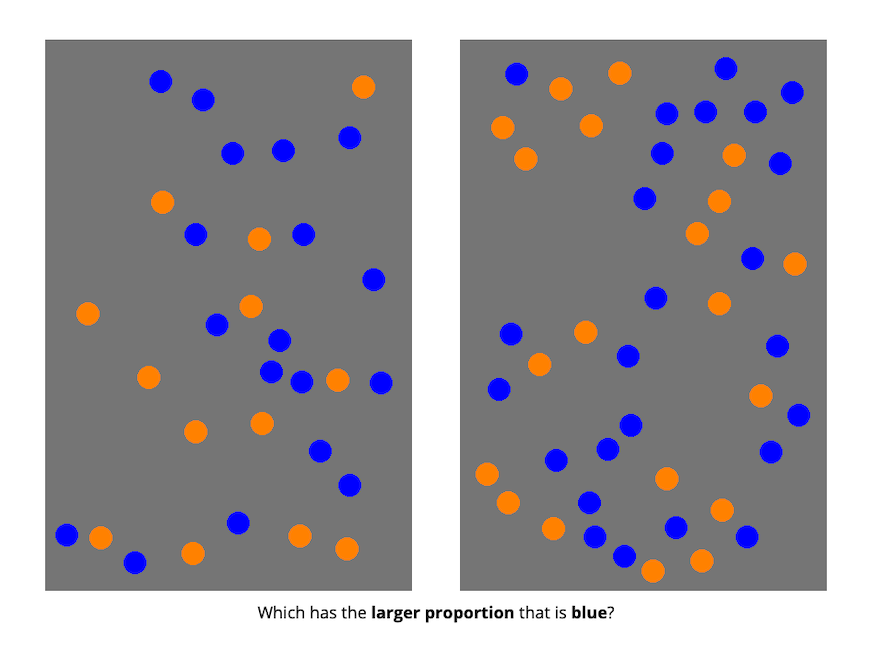
\includegraphics[width=1\linewidth]{img11/Probtask_Trial} 

}

\caption{ : An example of integrated blobs}\label{fig:img1}
\end{figure}

Conditions There were four different conditions that changed what kinds of images the participants saw:

\begin{itemize}
\tightlist
\item
  divided blobs: blur and orange were entirely separate.
\item
  integrated blob: one blob, divided to be part blue and part orange.
\item
  separated dots: blue and orange dots were on opposite sides of the image.
\item
  integrated dots: blue and orange dots were intermixed.
\end{itemize}

\begin{figure}

{\centering 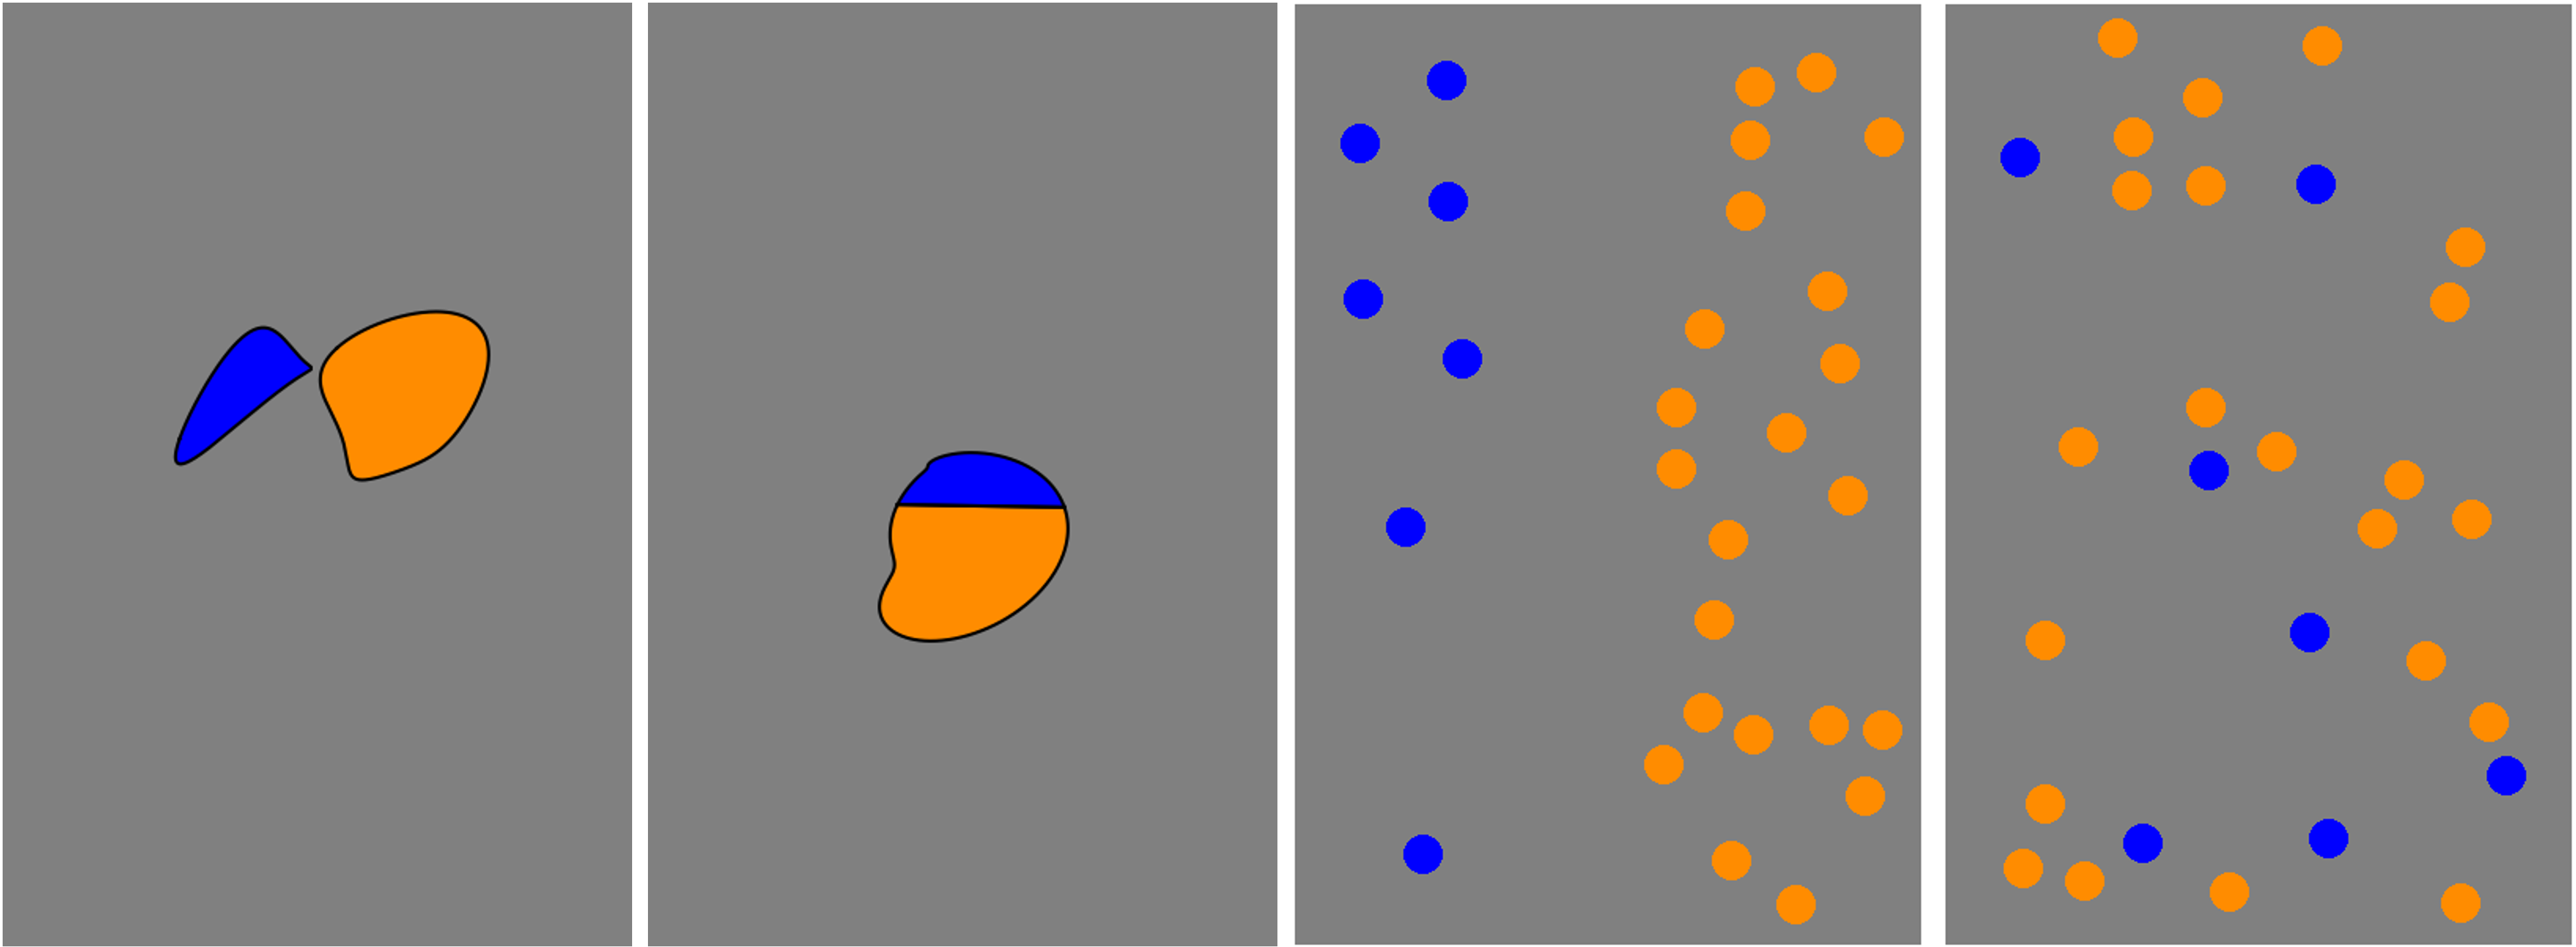
\includegraphics[width=1\linewidth]{img11/Probtask_formats} 

}

\caption{ From left to right : divided blobs, integrated blobs, separated dots, integraed dots}\label{fig:img2}
\end{figure}

\newpage

\section{Results}\label{results}

\begin{enumerate}
\def\labelenumi{\arabic{enumi}.}
\tightlist
\item
  Does average performance vary across format type, ignoring all other aspects of the stimuli?
\end{enumerate}

\begin{figure}

{\centering 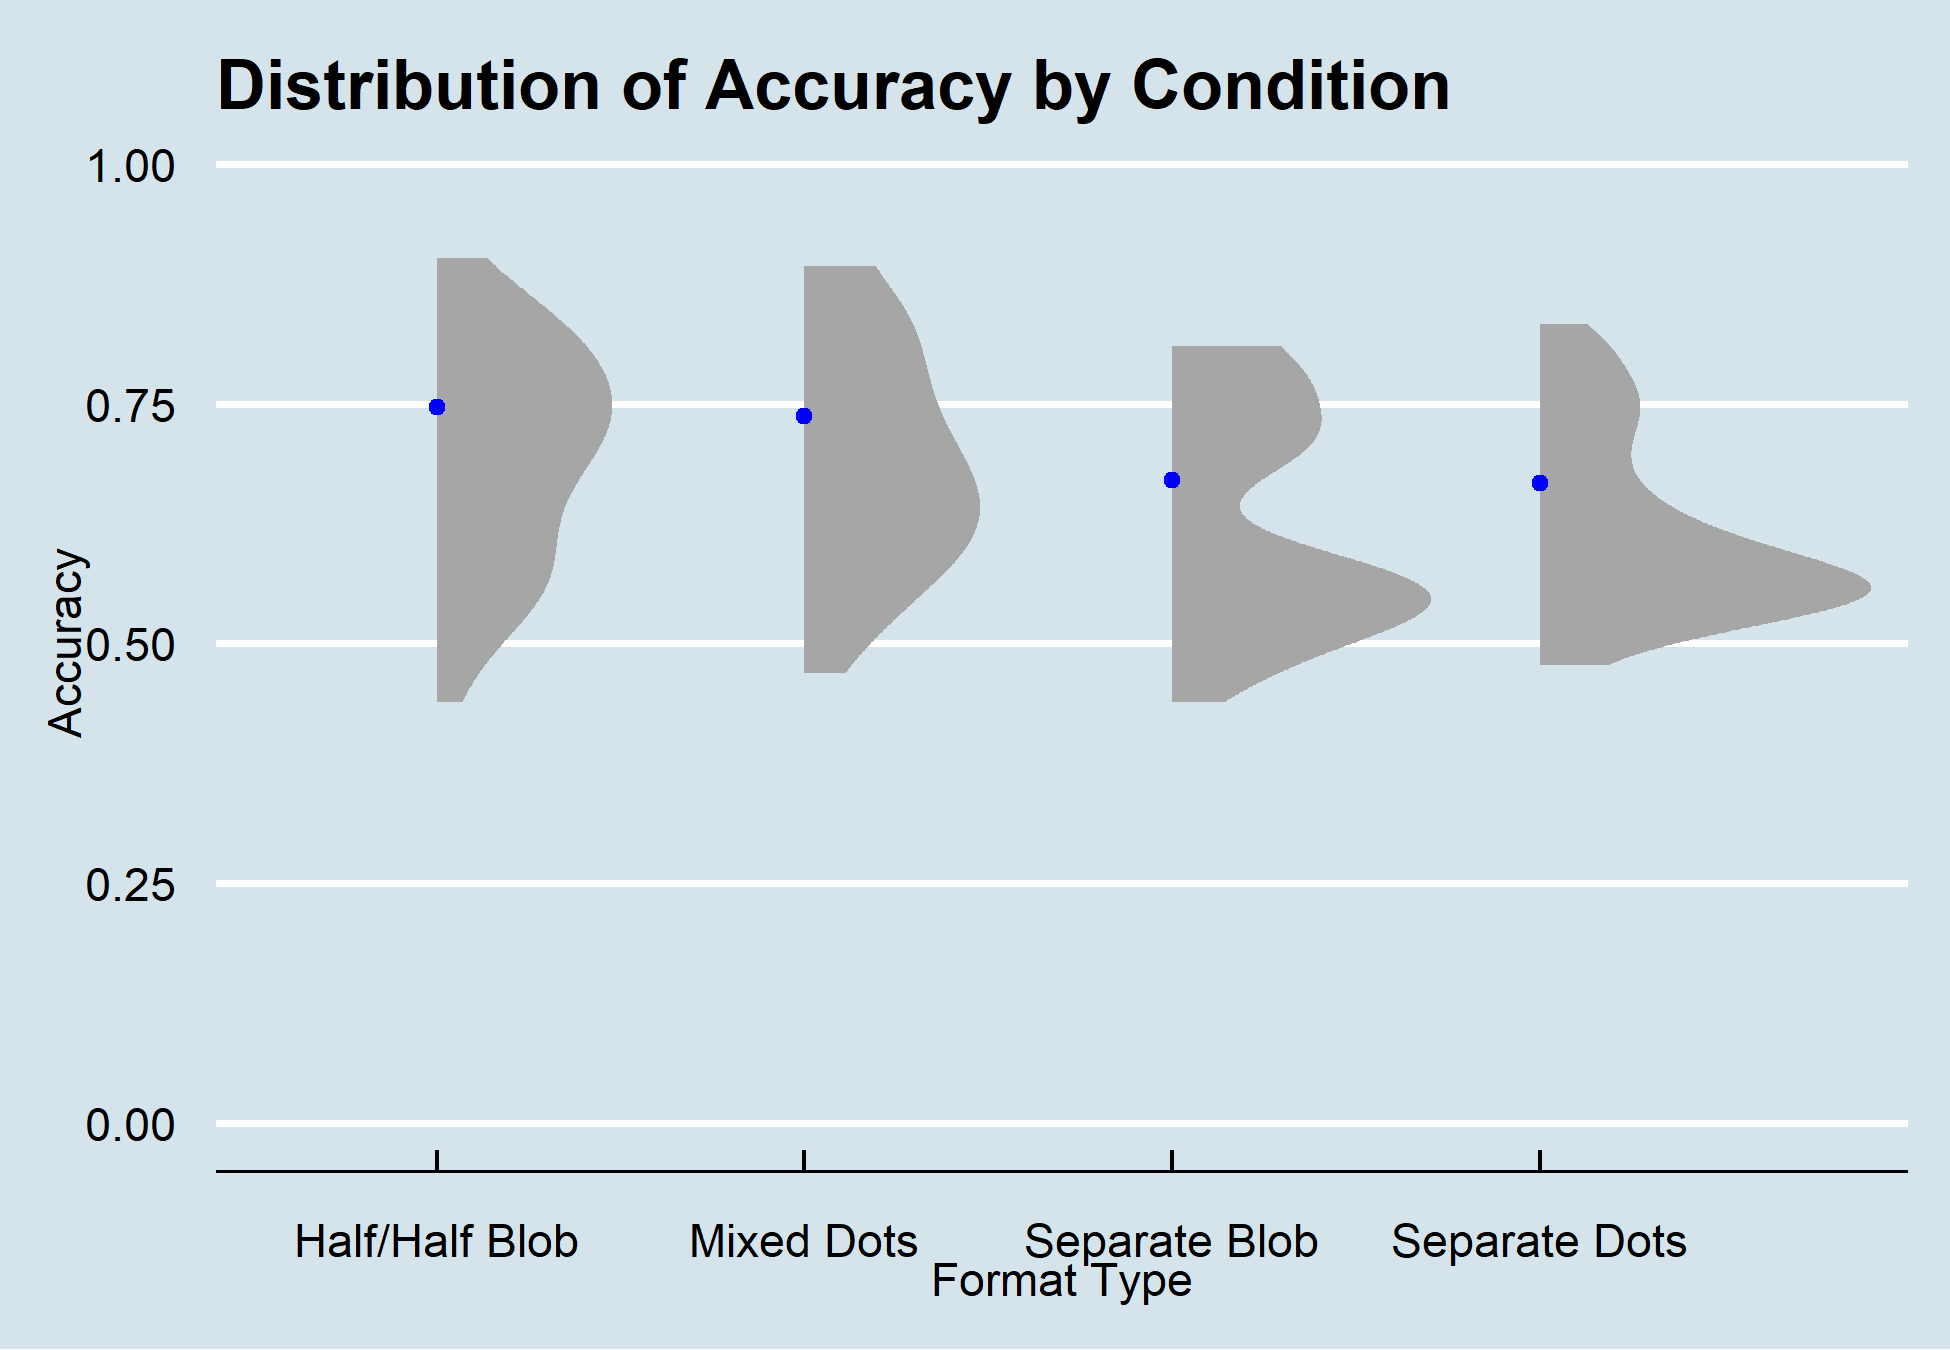
\includegraphics[width=1\linewidth]{Chin_WA11_files/figure-latex/returnplot-1} 

}

\caption{Plot of Distribution of Accuracy by Condition}\label{fig:returnplot}
\end{figure}

\emph{Yes, the blue dots in the above plot prove that the average performance varies across formatting types.}

list(condition = c(``blob\_shifted'', ``blob\_shifted'', ``blob\_shifted'', ``blob\_shifted'', ``blob\_shifted'', ``blob\_shifted'', ``blob\_shifted'', ``blob\_shifted'', ``blob\_shifted'', ``blob\_shifted'', ``blob\_shifted'', ``blob\_shifted'', ``blob\_shifted'', ``blob\_shifted'', ``blob\_shifted'', ``blob\_shifted'', ``blob\_shifted'', ``blob\_shifted'', ``blob\_shifted'', ``blob\_shifted'', ``blob\_shifted'', ``blob\_shifted'', ``blob\_shifted'', ``blob\_shifted'', ``blob\_shifted'', ``blob\_shifted'', ``blob\_shifted'', ``blob\_shifted'', ``blob\_shifted'', ``blob\_shifted'', ``blob\_shifted'',
``blob\_shifted'', ``blob\_shifted'', ``blob\_shifted'', ``blob\_shifted'', ``blob\_shifted'', ``blob\_shifted'', ``blob\_shifted'', ``blob\_shifted'', ``blob\_shifted'', ``blob\_shifted'', ``blob\_shifted'', ``blob\_shifted'', ``blob\_shifted'', ``blob\_shifted'', ``blob\_shifted'', ``blob\_shifted'', ``blob\_shifted'', ``blob\_shifted'', ``blob\_shifted'', ``blob\_stacked'', ``blob\_stacked'', ``blob\_stacked'', ``blob\_stacked'', ``blob\_stacked'', ``blob\_stacked'', ``blob\_stacked'', ``blob\_stacked'', ``blob\_stacked'', ``blob\_stacked'', ``blob\_stacked'', ``blob\_stacked'', ``blob\_stacked'',
``blob\_stacked'', ``blob\_stacked'', ``blob\_stacked'', ``blob\_stacked'', ``blob\_stacked'', ``blob\_stacked'', ``blob\_stacked'', ``blob\_stacked'', ``blob\_stacked'', ``blob\_stacked'', ``blob\_stacked'', ``blob\_stacked'', ``blob\_stacked'', ``blob\_stacked'', ``blob\_stacked'', ``blob\_stacked'', ``blob\_stacked'', ``blob\_stacked'', ``blob\_stacked'', ``blob\_stacked'', ``blob\_stacked'', ``blob\_stacked'', ``blob\_stacked'', ``blob\_stacked'', ``blob\_stacked'', ``blob\_stacked'', ``blob\_stacked'', ``blob\_stacked'', ``blob\_stacked'', ``blob\_stacked'', ``blob\_stacked'', ``blob\_stacked'',
``blob\_stacked'', ``blob\_stacked'', ``blob\_stacked'', ``blob\_stacked'', ``blob\_stacked'', ``dots\_EqSizeRand'', ``dots\_EqSizeRand'', ``dots\_EqSizeRand'', ``dots\_EqSizeRand'', ``dots\_EqSizeRand'', ``dots\_EqSizeRand'', ``dots\_EqSizeRand'', ``dots\_EqSizeRand'', ``dots\_EqSizeRand'', ``dots\_EqSizeRand'', ``dots\_EqSizeRand'', ``dots\_EqSizeRand'', ``dots\_EqSizeRand'', ``dots\_EqSizeRand'', ``dots\_EqSizeRand'', ``dots\_EqSizeRand'', ``dots\_EqSizeRand'', ``dots\_EqSizeRand'', ``dots\_EqSizeRand'', ``dots\_EqSizeRand'', ``dots\_EqSizeRand'', ``dots\_EqSizeRand'', ``dots\_EqSizeRand'',
``dots\_EqSizeRand'', ``dots\_EqSizeRand'', ``dots\_EqSizeRand'', ``dots\_EqSizeRand'', ``dots\_EqSizeRand'', ``dots\_EqSizeRand'', ``dots\_EqSizeRand'', ``dots\_EqSizeRand'', ``dots\_EqSizeRand'', ``dots\_EqSizeRand'', ``dots\_EqSizeRand'', ``dots\_EqSizeRand'', ``dots\_EqSizeRand'', ``dots\_EqSizeRand'', ``dots\_EqSizeRand'', ``dots\_EqSizeRand'', ``dots\_EqSizeRand'', ``dots\_EqSizeRand'', ``dots\_EqSizeRand'', ``dots\_EqSizeRand'', ``dots\_EqSizeRand'', ``dots\_EqSizeRand'', ``dots\_EqSizeRand'', ``dots\_EqSizeRand'', ``dots\_EqSizeRand'', ``dots\_EqSizeRand'', ``dots\_EqSizeSep'',
``dots\_EqSizeSep'', ``dots\_EqSizeSep'', ``dots\_EqSizeSep'', ``dots\_EqSizeSep'', ``dots\_EqSizeSep'', ``dots\_EqSizeSep'', ``dots\_EqSizeSep'', ``dots\_EqSizeSep'', ``dots\_EqSizeSep'', ``dots\_EqSizeSep'', ``dots\_EqSizeSep'', ``dots\_EqSizeSep'', ``dots\_EqSizeSep'', ``dots\_EqSizeSep'', ``dots\_EqSizeSep'', ``dots\_EqSizeSep'', ``dots\_EqSizeSep'', ``dots\_EqSizeSep'', ``dots\_EqSizeSep'', ``dots\_EqSizeSep'', ``dots\_EqSizeSep'', ``dots\_EqSizeSep'', ``dots\_EqSizeSep'', ``dots\_EqSizeSep'', ``dots\_EqSizeSep'', ``dots\_EqSizeSep'', ``dots\_EqSizeSep'', ``dots\_EqSizeSep'',
``dots\_EqSizeSep'', ``dots\_EqSizeSep'', ``dots\_EqSizeSep'', ``dots\_EqSizeSep'', ``dots\_EqSizeSep'', ``dots\_EqSizeSep'', ``dots\_EqSizeSep'', ``dots\_EqSizeSep'', ``dots\_EqSizeSep'', ``dots\_EqSizeSep'', ``dots\_EqSizeSep'', ``dots\_EqSizeSep'', ``dots\_EqSizeSep'', ``dots\_EqSizeSep'', ``dots\_EqSizeSep'', ``dots\_EqSizeSep'', ``dots\_EqSizeSep'', ``dots\_EqSizeSep'', ``dots\_EqSizeSep'', ``dots\_EqSizeSep''), mean\_prop\_corr = c(0.620151515151515, 0.620151515151515, 0.620151515151515, 0.620151515151515, 0.620151515151515, 0.620151515151515, 0.620151515151515,
0.620151515151515, 0.620151515151515, 0.620151515151515, 0.620151515151515, 0.620151515151515, 0.620151515151515, 0.620151515151515, 0.620151515151515, 0.620151515151515, 0.620151515151515, 0.620151515151515, 0.620151515151515, 0.620151515151515, 0.620151515151515, 0.620151515151515, 0.620151515151515, 0.620151515151515, 0.620151515151515, 0.620151515151515, 0.620151515151515, 0.620151515151515, 0.620151515151515, 0.620151515151515, 0.620151515151515, 0.620151515151515, 0.620151515151515, 0.620151515151515,
0.620151515151515, 0.620151515151515, 0.620151515151515, 0.620151515151515, 0.620151515151515, 0.620151515151515, 0.620151515151515, 0.620151515151515, 0.620151515151515, 0.620151515151515, 0.620151515151515, 0.620151515151515, 0.620151515151515, 0.620151515151515, 0.620151515151515, 0.620151515151515, 0.696666666666667, 0.696666666666667, 0.696666666666667, 0.696666666666667, 0.696666666666667, 0.696666666666667, 0.696666666666667, 0.696666666666667, 0.696666666666667, 0.696666666666667, 0.696666666666667,
0.696666666666667, 0.696666666666667, 0.696666666666667, 0.696666666666667, 0.696666666666667, 0.696666666666667, 0.696666666666667, 0.696666666666667, 0.696666666666667, 0.696666666666667, 0.696666666666667, 0.696666666666667, 0.696666666666667, 0.696666666666667, 0.696666666666667, 0.696666666666667, 0.696666666666667, 0.696666666666667, 0.696666666666667, 0.696666666666667, 0.696666666666667, 0.696666666666667, 0.696666666666667, 0.696666666666667, 0.696666666666667, 0.696666666666667, 0.696666666666667,
0.696666666666667, 0.696666666666667, 0.696666666666667, 0.696666666666667, 0.696666666666667, 0.696666666666667, 0.696666666666667, 0.696666666666667, 0.696666666666667, 0.696666666666667, 0.696666666666667, 0.696666666666667, 0.687384044526902, 0.687384044526902, 0.687384044526902, 0.687384044526902, 0.687384044526902, 0.687384044526902, 0.687384044526902, 0.687384044526902, 0.687384044526902, 0.687384044526902, 0.687384044526902, 0.687384044526902, 0.687384044526902, 0.687384044526902, 0.687384044526902,
0.687384044526902, 0.687384044526902, 0.687384044526902, 0.687384044526902, 0.687384044526902, 0.687384044526902, 0.687384044526902, 0.687384044526902, 0.687384044526902, 0.687384044526902, 0.687384044526902, 0.687384044526902, 0.687384044526902, 0.687384044526902, 0.687384044526902, 0.687384044526902, 0.687384044526902, 0.687384044526902, 0.687384044526902, 0.687384044526902, 0.687384044526902, 0.687384044526902, 0.687384044526902, 0.687384044526902, 0.687384044526902, 0.687384044526902, 0.687384044526902,
0.687384044526902, 0.687384044526902, 0.687384044526902, 0.687384044526902, 0.687384044526902, 0.687384044526902, 0.687384044526902, 0.617656153370439, 0.617656153370439, 0.617656153370439, 0.617656153370439, 0.617656153370439, 0.617656153370439, 0.617656153370439, 0.617656153370439, 0.617656153370439, 0.617656153370439, 0.617656153370439, 0.617656153370439, 0.617656153370439, 0.617656153370439, 0.617656153370439, 0.617656153370439, 0.617656153370439, 0.617656153370439, 0.617656153370439, 0.617656153370439,
0.617656153370439, 0.617656153370439, 0.617656153370439, 0.617656153370439, 0.617656153370439, 0.617656153370439, 0.617656153370439, 0.617656153370439, 0.617656153370439, 0.617656153370439, 0.617656153370439, 0.617656153370439, 0.617656153370439, 0.617656153370439, 0.617656153370439, 0.617656153370439, 0.617656153370439, 0.617656153370439, 0.617656153370439, 0.617656153370439, 0.617656153370439, 0.617656153370439, 0.617656153370439, 0.617656153370439, 0.617656153370439, 0.617656153370439, 0.617656153370439,
0.617656153370439, 0.617656153370439), sd\_prop\_corr = c(0.10993252708132, 0.10993252708132, 0.10993252708132, 0.10993252708132, 0.10993252708132, 0.10993252708132, 0.10993252708132, 0.10993252708132, 0.10993252708132, 0.10993252708132, 0.10993252708132, 0.10993252708132, 0.10993252708132, 0.10993252708132, 0.10993252708132, 0.10993252708132, 0.10993252708132, 0.10993252708132, 0.10993252708132, 0.10993252708132, 0.10993252708132, 0.10993252708132, 0.10993252708132, 0.10993252708132, 0.10993252708132,
0.10993252708132, 0.10993252708132, 0.10993252708132, 0.10993252708132, 0.10993252708132, 0.10993252708132, 0.10993252708132, 0.10993252708132, 0.10993252708132, 0.10993252708132, 0.10993252708132, 0.10993252708132, 0.10993252708132, 0.10993252708132, 0.10993252708132, 0.10993252708132, 0.10993252708132, 0.10993252708132, 0.10993252708132, 0.10993252708132, 0.10993252708132, 0.10993252708132, 0.10993252708132, 0.10993252708132, 0.10993252708132, 0.11390876441947, 0.11390876441947, 0.11390876441947,
0.11390876441947, 0.11390876441947, 0.11390876441947, 0.11390876441947, 0.11390876441947, 0.11390876441947, 0.11390876441947, 0.11390876441947, 0.11390876441947, 0.11390876441947, 0.11390876441947, 0.11390876441947, 0.11390876441947, 0.11390876441947, 0.11390876441947, 0.11390876441947, 0.11390876441947, 0.11390876441947, 0.11390876441947, 0.11390876441947, 0.11390876441947, 0.11390876441947, 0.11390876441947, 0.11390876441947, 0.11390876441947, 0.11390876441947, 0.11390876441947, 0.11390876441947,
0.11390876441947, 0.11390876441947, 0.11390876441947, 0.11390876441947, 0.11390876441947, 0.11390876441947, 0.11390876441947, 0.11390876441947, 0.11390876441947, 0.11390876441947, 0.11390876441947, 0.11390876441947, 0.11390876441947, 0.11390876441947, 0.11390876441947, 0.11390876441947, 0.11390876441947, 0.11390876441947, 0.11390876441947, 0.11090763670387, 0.11090763670387, 0.11090763670387, 0.11090763670387, 0.11090763670387, 0.11090763670387, 0.11090763670387, 0.11090763670387, 0.11090763670387,
0.11090763670387, 0.11090763670387, 0.11090763670387, 0.11090763670387, 0.11090763670387, 0.11090763670387, 0.11090763670387, 0.11090763670387, 0.11090763670387, 0.11090763670387, 0.11090763670387, 0.11090763670387, 0.11090763670387, 0.11090763670387, 0.11090763670387, 0.11090763670387, 0.11090763670387, 0.11090763670387, 0.11090763670387, 0.11090763670387, 0.11090763670387, 0.11090763670387, 0.11090763670387, 0.11090763670387, 0.11090763670387, 0.11090763670387, 0.11090763670387, 0.11090763670387,
0.11090763670387, 0.11090763670387, 0.11090763670387, 0.11090763670387, 0.11090763670387, 0.11090763670387, 0.11090763670387, 0.11090763670387, 0.11090763670387, 0.11090763670387, 0.11090763670387, 0.11090763670387, 0.0940521231301154, 0.0940521231301154, 0.0940521231301154, 0.0940521231301154, 0.0940521231301154, 0.0940521231301154, 0.0940521231301154, 0.0940521231301154, 0.0940521231301154, 0.0940521231301154, 0.0940521231301154, 0.0940521231301154, 0.0940521231301154, 0.0940521231301154, 0.0940521231301154,
0.0940521231301154, 0.0940521231301154, 0.0940521231301154, 0.0940521231301154, 0.0940521231301154, 0.0940521231301154, 0.0940521231301154, 0.0940521231301154, 0.0940521231301154, 0.0940521231301154, 0.0940521231301154, 0.0940521231301154, 0.0940521231301154, 0.0940521231301154, 0.0940521231301154, 0.0940521231301154, 0.0940521231301154, 0.0940521231301154, 0.0940521231301154, 0.0940521231301154, 0.0940521231301154, 0.0940521231301154, 0.0940521231301154, 0.0940521231301154, 0.0940521231301154, 0.0940521231301154,
0.0940521231301154, 0.0940521231301154, 0.0940521231301154, 0.0940521231301154, 0.0940521231301154, 0.0940521231301154, 0.0940521231301154, 0.0940521231301154), prop\_corr = c(0.46969696969697, 0.53030303030303, 0.583333333333333, 0.545454545454545, 0.75, 0.795454545454545, 0.583333333333333, 0.5, 0.795454545454545, 0.757575757575758, 0.575757575757576, 0.553030303030303, 0.583333333333333, 0.712121212121212, 0.628787878787879, 0.5, 0.696969696969697, 0.71969696969697, 0.46969696969697, 0.71969696969697,
0.545454545454545, 0.704545454545455, 0.568181818181818, 0.46969696969697, 0.5, 0.568181818181818, 0.553030303030303, 0.515151515151515, 0.757575757575758, 0.575757575757576, 0.71969696969697, 0.757575757575758, 0.742424242424242, 0.537878787878788, 0.522727272727273, 0.537878787878788, 0.537878787878788, 0.803030303030303, 0.810606060606061, 0.568181818181818, 0.787878787878788, 0.689393939393939, 0.439393939393939, 0.681818181818182, 0.598484848484849, 0.545454545454545, 0.515151515151515, 0.666666666666667,
0.53030303030303, 0.787878787878788, 0.704545454545455, 0.704545454545455, 0.712121212121212, 0.613636363636364, 0.863636363636364, 0.856060606060606, 0.666666666666667, 0.439393939393939, 0.856060606060606, 0.803030303030303, 0.787878787878788, 0.643939393939394, 0.734848484848485, 0.742424242424242, 0.704545454545455, 0.712121212121212, 0.659090909090909, 0.810606060606061, 0.590909090909091, 0.742424242424242, 0.704545454545455, 0.765151515151515, 0.53030303030303, 0.643939393939394, 0.553030303030303,
0.583333333333333, 0.560606060606061, 0.590909090909091, 0.840909090909091, 0.537878787878788, 0.901515151515151, 0.810606060606061, 0.840909090909091, 0.757575757575758, 0.583333333333333, 0.46969696969697, 0.613636363636364, 0.803030303030303, 0.78030303030303, 0.545454545454545, 0.818181818181818, 0.803030303030303, 0.53030303030303, 0.787878787878788, 0.659090909090909, 0.704545454545455, 0.545454545454545, 0.757575757575758, 0.734848484848485, 0.727272727272727, 0.46969696969697, 0.681818181818182,
0.5, 0.590909090909091, 0.598484848484849, 0.53030303030303, 0.666666666666667, 0.893939393939394, 0.727272727272727, 0.742424242424242, 0.795454545454545, 0.53030303030303, 0.772727272727273, 0.825757575757576, 0.704545454545455, 0.674242424242424, 0.53030303030303, 0.681818181818182, 0.765151515151515, 0.825757575757576, 0.863636363636364, 0.659090909090909, 0.871212121212121, 0.833333333333333, 0.810606060606061, 0.598484848484849, 0.598484848484849, 0.787878787878788, 0.560606060606061, 0.666666666666667,
0.659090909090909, 0.636363636363636, 0.674242424242424, 0.666666666666667, 0.757575757575758, 0.727272727272727, 0.712121212121212, 0.734848484848485, 0.537878787878788, 0.628787878787879, 0.598484848484849, 0.613636363636364, 0.590909090909091, 0.863636363636364, 0.863636363636364, 0.606060606060606, 0.825757575757576, 0.613636363636364, 0.613636363636364, 0.666666666666667, 0.537878787878788, 0.53030303030303, 0.568181818181818, 0.810606060606061, 0.575757575757576, 0.575757575757576, 0.787878787878788,
0.696969696969697, 0.71969696969697, 0.553030303030303, 0.598484848484849, 0.833333333333333, 0.575757575757576, 0.704545454545455, 0.545454545454545, 0.477272727272727, 0.568181818181818, 0.575757575757576, 0.651515151515151, 0.772727272727273, 0.553030303030303, 0.742424242424242, 0.613636363636364, 0.734848484848485, 0.606060606060606, 0.53030303030303, 0.757575757575758, 0.583333333333333, 0.537878787878788, 0.590909090909091, 0.621212121212121, 0.643939393939394, 0.560606060606061, 0.545454545454545,
0.628787878787879, 0.621212121212121, 0.484848484848485, 0.583333333333333, 0.537878787878788, 0.507575757575758, 0.537878787878788, 0.553030303030303, 0.810606060606061, 0.674242424242424, 0.545454545454545, 0.757575757575758, 0.553030303030303, 0.522727272727273), n = c(50, 50, 50, 50, 50, 50, 50, 50, 50, 50, 50, 50, 50, 50, 50, 50, 50, 50, 50, 50, 50, 50, 50, 50, 50, 50, 50, 50, 50, 50, 50, 50, 50, 50, 50, 50, 50, 50, 50, 50, 50, 50, 50, 50, 50, 50, 50, 50, 50, 50, 50, 50, 50, 50, 50, 50, 50,
50, 50, 50, 50, 50, 50, 50, 50, 50, 50, 50, 50, 50, 50, 50, 50, 50, 50, 50, 50, 50, 50, 50, 50, 50, 50, 50, 50, 50, 50, 50, 50, 50, 50, 50, 50, 50, 50, 50, 50, 50, 50, 50, 49, 49, 49, 49, 49, 49, 49, 49, 49, 49, 49, 49, 49, 49, 49, 49, 49, 49, 49, 49, 49, 49, 49, 49, 49, 49, 49, 49, 49, 49, 49, 49, 49, 49, 49, 49, 49, 49, 49, 49, 49, 49, 49, 49, 49, 49, 49, 49, 49, 49, 49, 49, 49, 49, 49, 49, 49, 49, 49, 49, 49, 49, 49, 49, 49, 49, 49, 49, 49, 49, 49, 49, 49, 49, 49, 49, 49, 49, 49, 49, 49, 49, 49,
49, 49, 49, 49, 49, 49, 49, 49, 49, 49, 49, 49, 49, 49, 49), condition\_name = c(``Separate Blob'', ``Separate Blob'', ``Separate Blob'', ``Separate Blob'', ``Separate Blob'', ``Separate Blob'', ``Separate Blob'', ``Separate Blob'', ``Separate Blob'', ``Separate Blob'', ``Separate Blob'', ``Separate Blob'', ``Separate Blob'', ``Separate Blob'', ``Separate Blob'', ``Separate Blob'', ``Separate Blob'', ``Separate Blob'', ``Separate Blob'', ``Separate Blob'', ``Separate Blob'', ``Separate Blob'', ``Separate Blob'', ``Separate Blob'', ``Separate Blob'',
``Separate Blob'', ``Separate Blob'', ``Separate Blob'', ``Separate Blob'', ``Separate Blob'', ``Separate Blob'', ``Separate Blob'', ``Separate Blob'', ``Separate Blob'', ``Separate Blob'', ``Separate Blob'', ``Separate Blob'', ``Separate Blob'', ``Separate Blob'', ``Separate Blob'', ``Separate Blob'', ``Separate Blob'', ``Separate Blob'', ``Separate Blob'', ``Separate Blob'', ``Separate Blob'', ``Separate Blob'', ``Separate Blob'', ``Separate Blob'', ``Separate Blob'', ``Half/Half Blob'', ``Half/Half Blob'', ``Half/Half Blob'', ``Half/Half Blob'', ``Half/Half Blob'',
``Half/Half Blob'', ``Half/Half Blob'', ``Half/Half Blob'', ``Half/Half Blob'', ``Half/Half Blob'', ``Half/Half Blob'', ``Half/Half Blob'', ``Half/Half Blob'', ``Half/Half Blob'', ``Half/Half Blob'', ``Half/Half Blob'', ``Half/Half Blob'', ``Half/Half Blob'', ``Half/Half Blob'', ``Half/Half Blob'', ``Half/Half Blob'', ``Half/Half Blob'', ``Half/Half Blob'', ``Half/Half Blob'', ``Half/Half Blob'', ``Half/Half Blob'', ``Half/Half Blob'', ``Half/Half Blob'', ``Half/Half Blob'', ``Half/Half Blob'', ``Half/Half Blob'', ``Half/Half Blob'', ``Half/Half Blob'',
``Half/Half Blob'', ``Half/Half Blob'', ``Half/Half Blob'', ``Half/Half Blob'', ``Half/Half Blob'', ``Half/Half Blob'', ``Half/Half Blob'', ``Half/Half Blob'', ``Half/Half Blob'', ``Half/Half Blob'', ``Half/Half Blob'', ``Half/Half Blob'', ``Half/Half Blob'', ``Half/Half Blob'', ``Half/Half Blob'', ``Half/Half Blob'', ``Half/Half Blob'', ``Mixed Dots'', ``Mixed Dots'', ``Mixed Dots'', ``Mixed Dots'', ``Mixed Dots'', ``Mixed Dots'', ``Mixed Dots'', ``Mixed Dots'', ``Mixed Dots'', ``Mixed Dots'', ``Mixed Dots'', ``Mixed Dots'', ``Mixed Dots'', ``Mixed Dots'',
``Mixed Dots'', ``Mixed Dots'', ``Mixed Dots'', ``Mixed Dots'', ``Mixed Dots'', ``Mixed Dots'', ``Mixed Dots'', ``Mixed Dots'', ``Mixed Dots'', ``Mixed Dots'', ``Mixed Dots'', ``Mixed Dots'', ``Mixed Dots'', ``Mixed Dots'', ``Mixed Dots'', ``Mixed Dots'', ``Mixed Dots'', ``Mixed Dots'', ``Mixed Dots'', ``Mixed Dots'', ``Mixed Dots'', ``Mixed Dots'', ``Mixed Dots'', ``Mixed Dots'', ``Mixed Dots'', ``Mixed Dots'', ``Mixed Dots'', ``Mixed Dots'', ``Mixed Dots'', ``Mixed Dots'', ``Mixed Dots'', ``Mixed Dots'', ``Mixed Dots'', ``Mixed Dots'', ``Mixed Dots'', ``Separate Dots'',
``Separate Dots'', ``Separate Dots'', ``Separate Dots'', ``Separate Dots'', ``Separate Dots'', ``Separate Dots'', ``Separate Dots'', ``Separate Dots'', ``Separate Dots'', ``Separate Dots'', ``Separate Dots'', ``Separate Dots'', ``Separate Dots'', ``Separate Dots'', ``Separate Dots'', ``Separate Dots'', ``Separate Dots'', ``Separate Dots'', ``Separate Dots'', ``Separate Dots'', ``Separate Dots'', ``Separate Dots'', ``Separate Dots'', ``Separate Dots'', ``Separate Dots'', ``Separate Dots'', ``Separate Dots'', ``Separate Dots'', ``Separate Dots'', ``Separate Dots'',
``Separate Dots'', ``Separate Dots'', ``Separate Dots'', ``Separate Dots'', ``Separate Dots'', ``Separate Dots'', ``Separate Dots'', ``Separate Dots'', ``Separate Dots'', ``Separate Dots'', ``Separate Dots'', ``Separate Dots'', ``Separate Dots'', ``Separate Dots'', ``Separate Dots'', ``Separate Dots'', ``Separate Dots'', ``Separate Dots'')), list(, ), , , list(x = \textasciitilde condition\_name, y = \textasciitilde prop\_corr), list(line = list(colour = ``black'', linewidth = 0.5, linetype = 1, lineend = ``butt'', arrow = FALSE, inherit.blank = TRUE), rect = list(fill = ``white'', colour = ``black'', linewidth = 0.5, linetype = 1, inherit.blank = TRUE), text = list(family = ``\,``, face =''plain'', colour = ``black'', size = 11, hjust = 0.5, vjust = 0.5, angle = 0, lineheight = 0.9, margin = c(0, 0, 0, 0), debug = FALSE, inherit.blank = TRUE), title = NULL, aspect.ratio = NULL, axis.title = NULL, axis.title.x = list(family = NULL, face = NULL,
colour = NULL, size = NULL, hjust = NULL, vjust = 1, angle = NULL, lineheight = NULL, margin = c(2.75, 0, 0, 0), debug = NULL, inherit.blank = TRUE), axis.title.x.top = list(family = NULL, face = NULL, colour = NULL, size = NULL, hjust = NULL, vjust = 0, angle = NULL, lineheight = NULL, margin = c(0, 0, 2.75, 0), debug = NULL, inherit.blank = TRUE), axis.title.x.bottom = NULL, axis.title.y = list(family = NULL, face = NULL, colour = NULL, size = NULL, hjust = NULL, vjust = 1, angle = 90, lineheight = NULL,
margin = c(0, 2.75, 0, 0), debug = NULL, inherit.blank = TRUE), axis.title.y.left = NULL, axis.title.y.right = list(family = NULL, face = NULL, colour = NULL, size = NULL, hjust = NULL, vjust = 1, angle = -90, lineheight = NULL, margin = c(0, 0, 0, 2.75), debug = NULL, inherit.blank = TRUE), axis.text = list(family = NULL, face = NULL, colour = ``grey30'', size = 0.8, hjust = NULL, vjust = NULL, angle = NULL, lineheight = NULL, margin = NULL, debug = NULL, inherit.blank = TRUE), axis.text.x = list(
family = NULL, face = NULL, colour = NULL, size = NULL, hjust = NULL, vjust = 1, angle = NULL, lineheight = NULL, margin = c(2.2, 0, 0, 0), debug = NULL, inherit.blank = TRUE), axis.text.x.top = list(family = NULL, face = NULL, colour = NULL, size = NULL, hjust = NULL, vjust = 0, angle = NULL, lineheight = NULL, margin = c(0, 0, 2.2, 0), debug = NULL, inherit.blank = TRUE), axis.text.x.bottom = NULL, axis.text.y = list(family = NULL, face = NULL, colour = NULL, size = NULL, hjust = 1, vjust = NULL,
angle = NULL, lineheight = NULL, margin = c(0, 2.2, 0, 0), debug = NULL, inherit.blank = TRUE), axis.text.y.left = NULL, axis.text.y.right = list(family = NULL, face = NULL, colour = NULL, size = NULL, hjust = 0, vjust = NULL, angle = NULL, lineheight = NULL, margin = c(0, 0, 0, 2.2), debug = NULL, inherit.blank = TRUE), axis.text.theta = NULL, axis.text.r = list(family = NULL, face = NULL, colour = NULL, size = NULL, hjust = 0.5, vjust = NULL, angle = NULL, lineheight = NULL, margin = c(0, 2.2,
0, 2.2), debug = NULL, inherit.blank = TRUE), axis.ticks = list(), axis.ticks.x = NULL, axis.ticks.x.top = NULL, axis.ticks.x.bottom = NULL, axis.ticks.y = NULL, axis.ticks.y.left = NULL, axis.ticks.y.right = NULL, axis.ticks.theta = NULL, axis.ticks.r = NULL, axis.minor.ticks.x.top = NULL, axis.minor.ticks.x.bottom = NULL, axis.minor.ticks.y.left = NULL, axis.minor.ticks.y.right = NULL, axis.minor.ticks.theta = NULL, axis.minor.ticks.r = NULL, axis.ticks.length = 2.75, axis.ticks.length.x = NULL,
axis.ticks.length.x.top = NULL, axis.ticks.length.x.bottom = NULL, axis.ticks.length.y = NULL, axis.ticks.length.y.left = NULL, axis.ticks.length.y.right = NULL, axis.ticks.length.theta = NULL, axis.ticks.length.r = NULL, axis.minor.ticks.length = 0.75, axis.minor.ticks.length.x = NULL, axis.minor.ticks.length.x.top = NULL, axis.minor.ticks.length.x.bottom = NULL, axis.minor.ticks.length.y = NULL, axis.minor.ticks.length.y.left = NULL, axis.minor.ticks.length.y.right = NULL, axis.minor.ticks.length.theta = NULL,
axis.minor.ticks.length.r = NULL, axis.line = list(), axis.line.x = NULL, axis.line.x.top = NULL, axis.line.x.bottom = NULL, axis.line.y = NULL, axis.line.y.left = NULL, axis.line.y.right = NULL, axis.line.theta = NULL, axis.line.r = NULL, legend.background = list(), legend.margin = c(5.5, 5.5, 5.5, 5.5), legend.spacing = 11, legend.spacing.x = NULL, legend.spacing.y = NULL, legend.key = list(), legend.key.size = 1.2, legend.key.height = NULL, legend.key.width = NULL, legend.key.spacing = 5.5,
legend.key.spacing.x = NULL, legend.key.spacing.y = NULL, legend.frame = NULL, legend.ticks = NULL, legend.ticks.length = 0.2, legend.axis.line = NULL, legend.text = list(family = NULL, face = NULL, colour = NULL, size = 0.8, hjust = NULL, vjust = NULL, angle = NULL, lineheight = NULL, margin = NULL, debug = NULL, inherit.blank = TRUE), legend.text.position = NULL, legend.title = list(family = NULL, face = NULL, colour = NULL, size = NULL, hjust = 0, vjust = NULL, angle = NULL, lineheight = NULL,
margin = NULL, debug = NULL, inherit.blank = TRUE), legend.title.position = NULL, legend.position = ``right'', legend.position.inside = NULL, legend.direction = NULL, legend.byrow = NULL, legend.justification = ``center'', legend.justification.top = NULL, legend.justification.bottom = NULL, legend.justification.left = NULL, legend.justification.right = NULL, legend.justification.inside = NULL, legend.location = NULL, legend.box = NULL, legend.box.just = NULL, legend.box.margin = c(0, 0, 0, 0),
legend.box.background = list(), legend.box.spacing = 11, panel.background = list(), panel.border = list(), panel.spacing = 5.5, panel.spacing.x = NULL, panel.spacing.y = NULL, panel.grid = list(colour = ``grey92'', linewidth = NULL, linetype = NULL, lineend = NULL, arrow = FALSE, inherit.blank = TRUE), panel.grid.major = NULL, panel.grid.minor = list(colour = NULL, linewidth = 0.5, linetype = NULL, lineend = NULL, arrow = FALSE, inherit.blank = TRUE), panel.grid.major.x = NULL, panel.grid.major.y = NULL,
panel.grid.minor.x = NULL, panel.grid.minor.y = NULL, panel.ontop = FALSE, plot.background = list(), plot.title = list(family = NULL, face = NULL, colour = NULL, size = 1.2, hjust = 0, vjust = 1, angle = NULL, lineheight = NULL, margin = c(0, 0, 5.5, 0), debug = NULL, inherit.blank = TRUE), plot.title.position = ``panel'', plot.subtitle = list(family = NULL, face = NULL, colour = NULL, size = NULL, hjust = 0, vjust = 1, angle = NULL, lineheight = NULL, margin = c(0, 0, 5.5, 0), debug = NULL, inherit.blank = TRUE),
plot.caption = list(family = NULL, face = NULL, colour = NULL, size = 0.8, hjust = 1, vjust = 1, angle = NULL, lineheight = NULL, margin = c(5.5, 0, 0, 0), debug = NULL, inherit.blank = TRUE), plot.caption.position = ``panel'', plot.tag = list(family = NULL, face = NULL, colour = NULL, size = 1.2, hjust = 0.5, vjust = 0.5, angle = NULL, lineheight = NULL, margin = NULL, debug = NULL, inherit.blank = TRUE), plot.tag.position = ``topleft'', plot.tag.location = NULL, plot.margin = c(5.5, 5.5, 5.5, 5.5
), strip.background = list(), strip.background.x = NULL, strip.background.y = NULL, strip.clip = ``inherit'', strip.placement = ``inside'', strip.text = list(family = NULL, face = NULL, colour = ``grey10'', size = 0.8, hjust = NULL, vjust = NULL, angle = NULL, lineheight = NULL, margin = c(4.4, 4.4, 4.4, 4.4), debug = NULL, inherit.blank = TRUE), strip.text.x = NULL, strip.text.x.bottom = NULL, strip.text.x.top = NULL, strip.text.y = list(family = NULL, face = NULL, colour = NULL, size = NULL, hjust = NULL,
vjust = NULL, angle = -90, lineheight = NULL, margin = NULL, debug = NULL, inherit.blank = TRUE), strip.text.y.left = list(family = NULL, face = NULL, colour = NULL, size = NULL, hjust = NULL, vjust = NULL, angle = 90, lineheight = NULL, margin = NULL, debug = NULL, inherit.blank = TRUE), strip.text.y.right = NULL, strip.switch.pad.grid = 2.75, strip.switch.pad.wrap = 2.75), , , , , list(x = ``Format Type'', y = ``Accuracy'', title = ``Distribution of Accuracy by Condition'', xdist = ``xdist'', ydist = ``ydist'', dist = ``dist'', args = ``args'', arg1 = ``arg1'', arg2 = ``arg2'', arg3 = ``arg3'', arg4 = ``arg4'', arg5 = ``arg5'', arg6 = ``arg6'', arg7 = ``arg7'', arg8 = ``arg8'', arg9 = ``arg9'', weight = ``weight'', datatype = ``datatype'', thickness = ``f'')

\begin{enumerate}
\def\labelenumi{\arabic{enumi}.}
\setcounter{enumi}{1}
\item
  \newpage
\end{enumerate}

\subsection{Data analysis}\label{data-analysis}

We used R (Version 4.4.1; R Core Team, 2024) and the R-packages \emph{dplyr} (Version 1.1.4; Wickham, François, Henry, Müller, \& Vaughan, 2023), \emph{forcats} (Version 1.0.0; Wickham, 2023a), \emph{ggdist} (Version 3.3.2; Kay, 2024), \emph{ggplot2} (Version 3.5.1; Wickham, 2016), \emph{lubridate} (Version 1.9.3; Grolemund \& Wickham, 2011), \emph{papaja} (Version 0.1.3; Aust \& Barth, 2024), \emph{purrr} (Version 1.0.2; Wickham \& Henry, 2023), \emph{readr} (Version 2.1.5; Wickham, Hester, \& Bryan, 2024), \emph{stringr} (Version 1.5.1; Wickham, 2023b), \emph{tibble} (Version 3.2.1; Müller \& Wickham, 2023), \emph{tidyr} (Version 1.3.1; Wickham, Vaughan, \& Girlich, 2024), \emph{tidyverse} (Version 2.0.0; Wickham et al., 2019) and \emph{tinylabels} (Version 0.2.4; Barth, 2023) for all our analyses.

\section{Discussion}\label{discussion}

\newpage

\section{References}\label{references}

use r\_refs( file = ``references.bib'')

\phantomsection\label{refs}
\begin{CSLReferences}{1}{0}
\bibitem[\citeproctext]{ref-R-papaja}
Aust, F., \& Barth, M. (2024). \emph{{papaja}: {Prepare} reproducible {APA} journal articles with {R Markdown}}. \url{https://doi.org/10.32614/CRAN.package.papaja}

\bibitem[\citeproctext]{ref-R-tinylabels}
Barth, M. (2023). \emph{{tinylabels}: Lightweight variable labels}. Retrieved from \url{https://cran.r-project.org/package=tinylabels}

\bibitem[\citeproctext]{ref-R-lubridate}
Grolemund, G., \& Wickham, H. (2011). Dates and times made easy with {lubridate}. \emph{Journal of Statistical Software}, \emph{40}(3), 1--25. Retrieved from \url{https://www.jstatsoft.org/v40/i03/}

\bibitem[\citeproctext]{ref-R-ggdist}
Kay, M. (2024). {ggdist}: Visualizations of distributions and uncertainty in the grammar of graphics. \emph{IEEE Transactions on Visualization and Computer Graphics}, \emph{30}(1), 414--424. \url{https://doi.org/10.1109/TVCG.2023.3327195}

\bibitem[\citeproctext]{ref-R-tibble}
Müller, K., \& Wickham, H. (2023). \emph{Tibble: Simple data frames}. Retrieved from \url{https://CRAN.R-project.org/package=tibble}

\bibitem[\citeproctext]{ref-R-base}
R Core Team. (2024). \emph{R: A language and environment for statistical computing}. Vienna, Austria: R Foundation for Statistical Computing. Retrieved from \url{https://www.R-project.org/}

\bibitem[\citeproctext]{ref-R-ggplot2}
Wickham, H. (2016). \emph{ggplot2: Elegant graphics for data analysis}. Springer-Verlag New York. Retrieved from \url{https://ggplot2.tidyverse.org}

\bibitem[\citeproctext]{ref-R-forcats}
Wickham, H. (2023a). \emph{Forcats: Tools for working with categorical variables (factors)}. Retrieved from \url{https://CRAN.R-project.org/package=forcats}

\bibitem[\citeproctext]{ref-R-stringr}
Wickham, H. (2023b). \emph{Stringr: Simple, consistent wrappers for common string operations}. Retrieved from \url{https://CRAN.R-project.org/package=stringr}

\bibitem[\citeproctext]{ref-R-tidyverse}
Wickham, H., Averick, M., Bryan, J., Chang, W., McGowan, L. D., François, R., \ldots{} Yutani, H. (2019). Welcome to the {tidyverse}. \emph{Journal of Open Source Software}, \emph{4}(43), 1686. \url{https://doi.org/10.21105/joss.01686}

\bibitem[\citeproctext]{ref-R-dplyr}
Wickham, H., François, R., Henry, L., Müller, K., \& Vaughan, D. (2023). \emph{Dplyr: A grammar of data manipulation}. Retrieved from \url{https://CRAN.R-project.org/package=dplyr}

\bibitem[\citeproctext]{ref-R-purrr}
Wickham, H., \& Henry, L. (2023). \emph{Purrr: Functional programming tools}. Retrieved from \url{https://CRAN.R-project.org/package=purrr}

\bibitem[\citeproctext]{ref-R-readr}
Wickham, H., Hester, J., \& Bryan, J. (2024). \emph{Readr: Read rectangular text data}. Retrieved from \url{https://CRAN.R-project.org/package=readr}

\bibitem[\citeproctext]{ref-R-tidyr}
Wickham, H., Vaughan, D., \& Girlich, M. (2024). \emph{Tidyr: Tidy messy data}. Retrieved from \url{https://CRAN.R-project.org/package=tidyr}

\end{CSLReferences}


\end{document}
